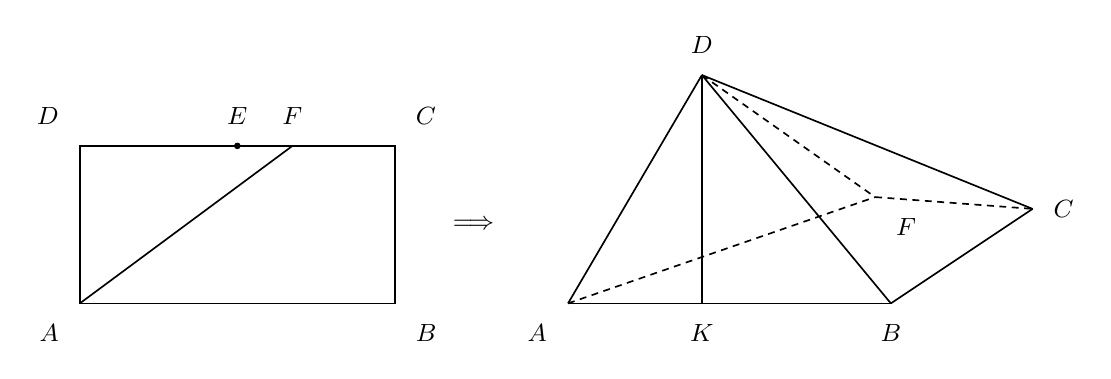
\begin{tikzpicture}[line width=0.6pt, font=\small]
% left panel: rectangle ABCD, E midpoint of DC, F on EC
\coordinate (A) at (0,0);
\coordinate (B) at (4,0);
\coordinate (C) at (4,2);
\coordinate (D) at (0,2);
\coordinate (E) at (2,2);
\coordinate (F) at (2.7,2);
\draw (A) -- (B) -- (C) -- (D) -- cycle;
\draw (A) -- (F);
\fill (E) circle (1.2pt);
\node[below left=4pt] at (A) {$A$};
\node[below right=4pt] at (B) {$B$};
\node[above right=4pt] at (C) {$C$};
\node[above left=4pt] at (D) {$D$};
\node[above=4pt] at (E) {$E$};
\node[above=4pt] at (F) {$F$};
\node at (5.0,1) {$\Longrightarrow$};
% right panel: folded pyramid D-A-B-C-F with DK vertical
\coordinate (A2) at (6.2,0);
\coordinate (K) at (7.9,0);
\coordinate (B2) at (10.3,0);
\coordinate (D2) at (7.9,2.9);
\coordinate (F2) at (10.1,1.35);
\coordinate (C2) at (12.1,1.2);
\draw (A2) -- (K) -- (B2);
\draw (A2) -- (D2);
\draw (D2) -- (K);
\draw (D2) -- (B2);
\draw (B2) -- (C2);
\draw (D2)--(C2);
\draw[dash pattern=on 2.5pt off 2pt] (A2) -- (F2);
\draw[dash pattern=on 2.5pt off 2pt] (D2) -- (F2);
\draw[dash pattern=on 2.5pt off 2pt] (F2) -- (C2);
\node[below left=4pt] at (A2) {$A$};
\node[below=4pt] at (K) {$K$};
\node[below=4pt] at (B2) {$B$};
\node[above=4pt] at (D2) {$D$};
\node[below right=4pt] at (F2) {$F$};
\node[right=4pt] at (C2) {$C$};
\end{tikzpicture}
